\chapter{Diseño de la interfaz} \label{cap:diseño_interfaz}

 \section{Introducción}

% En este capítulo se abordará el diseño de cada uno de los componentes que forman la interfaz de la aplicación. Puesto que muchos componentes son similares, se mostrará únicamente un componente de cada tipo. Un descripción más detallada de cada componente de la interfaz se puede consultar en el n el \textit{Manual de Usuario}.

% A continuación se muestran los elementos gráficos de la interfaz final de la aplicación con una explicación de cada una de las partes que los componen.

\section{Barras de menús}

% Las barras de menús contienen las acciones a realizar en una ventana agrupadas por categorías.
% En la figura \ref{fig:d1}, se muestra un ejemplo de una barra de menús para el Editor de gramáticas del programa SimAS.

%   \begin{figure}[htp]
%       \begin{center} 
% 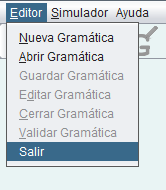
\includegraphics[width=0.2\textwidth]{figuras/Cap10/da2.png}
% 	\caption{Barras de menús de SimAS.}
% 	\label{fig:d1}
%       \end{center}
%   \end{figure}
  
%  La barra de menús contiene cada una de las acciones que se puede realizar en la aplicación SimAS agrupadas según la la funcionalidad de la acción. Además, se han dado nombres muy descriptivos a cada elemento, para así
% procurar que la interfaz sea lo más intuitiva posible. 

\section{Barras de herramientas}

% Las barras de herramientas contienen los accesos directos a las acciones que se pueden realizar en una ventana, que están representadas gráficamente. En la figura \ref{fig:d2}, se muestra un ejemplo de una barra de herramientas para la pantalla inicial del programa SimAS.

%   \begin{figure}[htp]
%       \begin{center} 
% 	
\includegraphics[width=0.5\textwidth]{figuras/Cap10/da4.png}
% 	\caption{Barra de herramientas de SimAS.}
% 	\label{fig:d2}
%       \end{center}
%   \end{figure}
  
%   Se ha procurado que cada botón sea descriptivo y represente fielmente la operación
% que realiza. Por esto, se ha tomado como convenio usar una forma base en 
% los iconos según el objeto al que involucran en la operación, por ejemplo: las operaciones de la gramática está representada con la letra \textit{G} y las operaciones de las simulaciones con la letra \textit{\textit{S}}. 

% A esta forma base, se le ha superpuesto una forma que representa de forma gráfica la acción a llevar a cabo. Así, se ha superpuesto la forma base del objeto con la acción a realizar, siempre en la esquina superior derecha de cada uno de los iconos de la barra de herramientas. Todo esto permite que la interfaz sea muy intuitiva y permita al usuario trabajar con eficacia y con el mínimo de confusiones posibles.
  

\section{Ventana del editor}

% La ventana del editor permite crear, editar y validar las gramáticas de contexto libre para su posterior simulación. 
% En la figura \ref{fig:d3}, se muestra un ejemplo de esta ventana con una gramática creada y validada.

% La ventana está compuesta de los siguientes elementos:
% \begin{enumerate}
%  \item \textbf{Barra de menús}: barra de menús de la ventana.
%  \item \textbf{Barra de herramientas}: barra de herramientas de la ventana.
%  \item \textbf{Panel de edición}: panel que almacena y representa las gramáticas.
% \end{enumerate}

%   \begin{figure}[htp]
%       \begin{center} 
% 	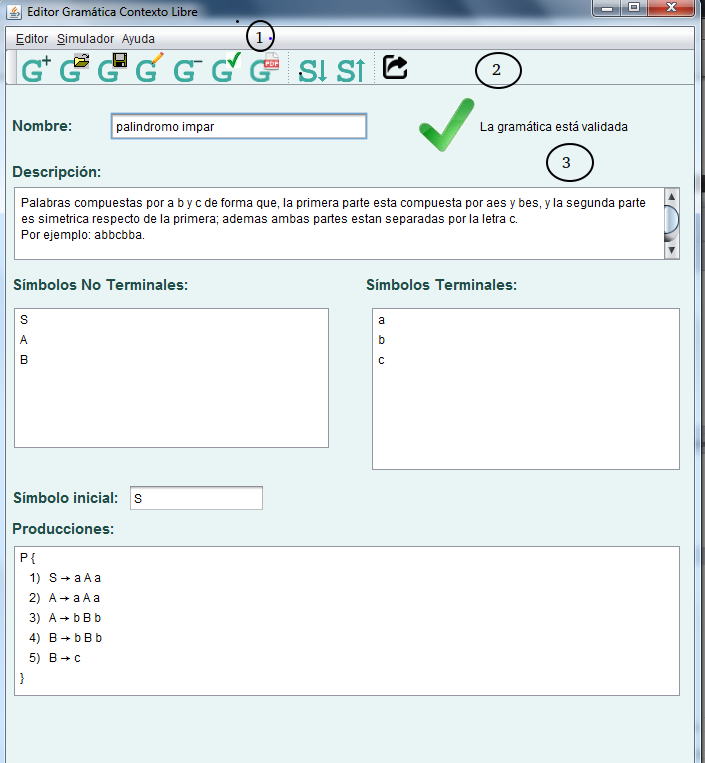
\includegraphics[width=0.6\textwidth]{figuras/Cap10/da6.png}
% 	\caption{Ventana del editor.}
% 	\label{fig:d3}
%       \end{center}
%   \end{figure}
  
%   En las secciones anteriores ya se vio con detalle la barra de menús y la barra de herramientas; a continuación se va a llevar a cabo la descripción de cada una de las partes que compone el panel de edición.

% \subsection{Panel de edición}

% El panel de edición permite visualizar cada uno de los componentes de las gramáticas de contexto libre así como su estado: validada o no validada. En la figura \ref{fig:d4}, se muestra un ejemplo de este panel.

% El panel está compuesto de los siguientes elementos:
% \begin{enumerate}
%  \item \textbf{Nombre de la gramática}: nombre descriptivo de la gramática.
%   \item \textbf{Estado de la gramática}: muestra si la gramática ha sido validada o no.
%   \item \textbf{Descripción}: descripción de la gramática.
%  \item \textbf{Símbolos de la gramática}: se muestran los símbolos terminales y los no terminales.
%  \item  \textbf{Símbolo inicial}: muestra cuál de los símbolos no terminales es el símbolo inicial de la gramática.
%  \item \textbf{Producciones de la gramática}: visualización de las reglas de producción de la gramática.
%  \end{enumerate}

%   \begin{figure}[htp]
%       \begin{center} 
% 	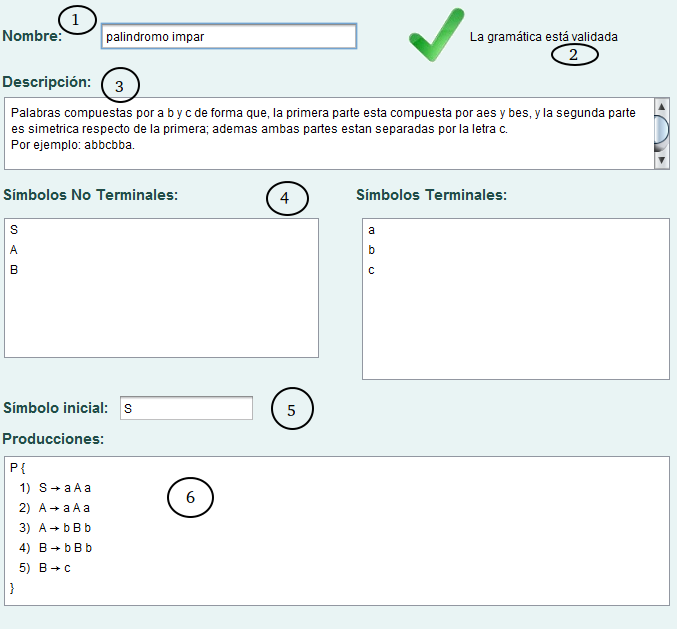
\includegraphics[width=0.5\textwidth]{figuras/Cap10/da8.png}
% 	\caption{Panel de edición}
% 	\label{fig:d4}
%       \end{center}
%   \end{figure}

\section{Ventana del simulador}

% La ventana del simulador permite ejecutar la simulación de un analizador descendente o ascendente utilizando una gramática. En la figura \ref{fig:d5}, se muestra un ejemplo de esta ventana.


% La ventana está compuesta de los siguientes elementos:
% \begin{enumerate}
%  \item \textbf{Barra de menús}: barra de menús de la ventana.
%  \item \textbf{Barra de herramientas}: barra de herramientas de la ventana.
%  \item \textbf{Panel de simulación}: panel que muestra los datos de la gramática a simular. 
% \end{enumerate}

%   \begin{figure}[htp]
%       \begin{center} 
% 	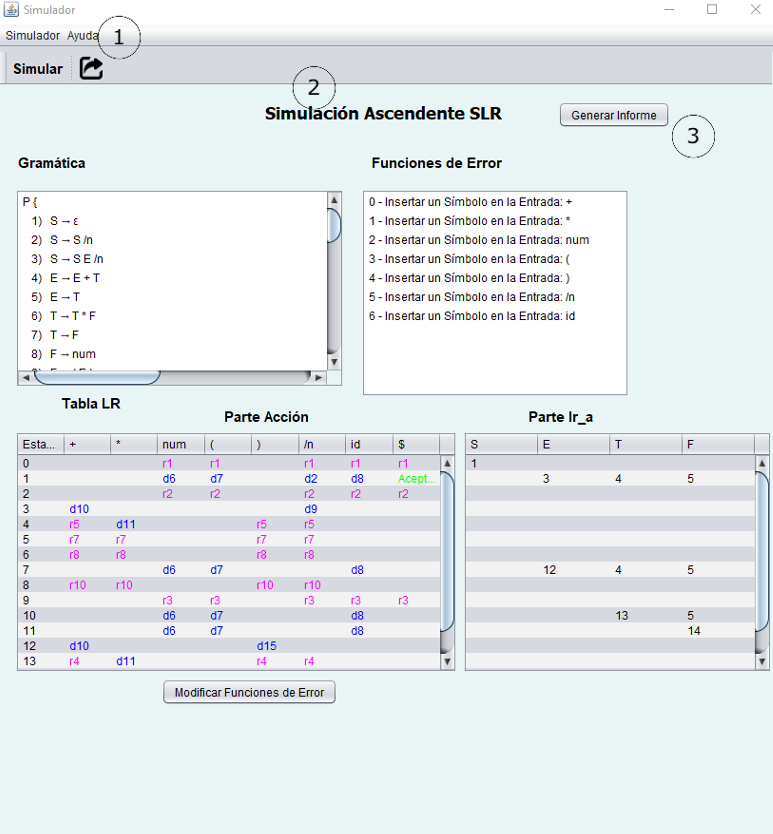
\includegraphics[width=0.6\textwidth]{figuras/Cap10/da10.png}
% 	\caption{ Ventana de simulación.}
% 	\label{fig:d5}
%       \end{center}
%   \end{figure}
  
%   En las secciones anteriores ya se vio con detalle la barra de menús y la barra de herramientas; a continuación, se llevará a cabo la descripción de cada una de las partes que compone el panel de simulación.



% \subsection{Panel de simulación}

% El panel de simulación permite visualizar las simulaciones de los analizadores sintácticos.
% En la figura \ref{fig:d6}, se muestra un ejemplo de este panel.

% El panel está compuesto de los siguientes elementos:
% \begin{enumerate}
%  \item \textbf{Tipo de análisis}: muestra el tipo de simulación que se va a llevar a cabo, \textit{descendente} o \textit{ascendente}. En el caso de ser la simulación del análisis ascendente, también se detalla el tipo: \textit{SLR}, \textit{LR-canónico} o \textit{LALR}.
%  \item \textbf{Producciones de la gramática}: visualización gráfica de las producciones de la gramática.
%  \item \textbf{Funciones de error}: lista de funciones de error de la gramática.
%  \item \textbf{Tabla predictiva o tabla LR}: muestra la tabla tabla predictiva o la tabla LR, dependiendo de método seleccionado.
% \end{enumerate}

%   \begin{figure}[htp]
%       \begin{center} 
% 	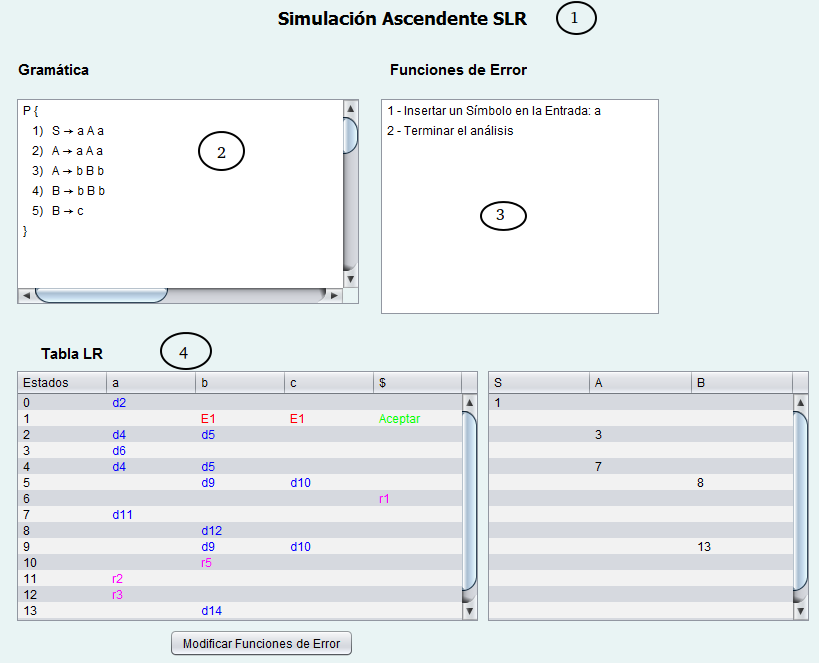
\includegraphics[width=0.6\textwidth]{figuras/Cap10/da12.png}
% 	\caption{ Panel de simulación}
% 	\label{fig:d6}
%       \end{center}
%   \end{figure}

% \subsection{Ventana de Gramática Original}

% \textbf{Visualización de la Gramática Original} (Novedad): a medida que se generan los diferentes conjuntos, tablas y funciones de error, se le permite al usuario visualizar la gramática original para así poder realizar las comparaciones que desee si dicha gramática se ha transformado en otra porque se ha eliminado la recursividad por la izquierda o se ha factorizado por la izquierda. 
% La ventana será un panel simple donde se muestre la gramática original de la misma forma que se muestra la gramática modificada (Figura \ref{fig:d10}).

%   \begin{figure}[htp]
%       \begin{center} 
% 	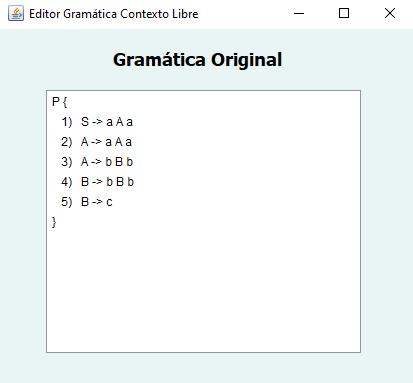
\includegraphics[width=0.5\textwidth]{figuras/Cap10/da20.PNG}
% 	\caption{ Gramática Original}
% 	\label{fig:d10}
%       \end{center}
%   \end{figure}

 \section{Ventana de simulación}

% La ventana de simulación se encarga de ejecutar las simulaciones de una cadena de entrada. 
% En la figura \ref{fig:d7}, se muestra un ejemplo de esta ventana.

% La ventana está compuesta de los siguientes elementos:
% \begin{enumerate}
%   \item \textbf{Tipo de análisis}: muestra el tipo de simulación que se va a llevar a cabo, \textit{descendente} o \textit{ascendente}. En el caso de ser la simulación del análisis ascendente, también se detalla el tipo: \textit{SLR}, \textit{LR-canónico} o \textit{LALR}.
%  \item \textbf{Cadena de entrada}: permite introducir los símbolos terminales que forman parte de la cadena de entrada que se va a simular.
%  \item \textbf{Botones de Avance y Retroceso}: la simulación se podrá realizar paso a paso o de forma completa, pudiendo avanzar y retroceder en cada paso.
%  \item \textbf{Tabla de análisis}: representa la tabla de resultados del análisis.
%  \item \textbf{Generar Árbol Sintáctico} (Novedad): permite abrir una ventana en la que se genere el árbol sintáctico correspondiente.
%  \item \textbf{Generar Derivación} (Novedad): permite abrir una ventana en la que se genere la derivación de la simulación correspondiente.
%  \item \textbf{Informe de la Simulación}: permite al usuario generar un informe en pdf de la simulación.

% \end{enumerate}

%   \begin{figure}[htp]
%       \begin{center} 
% 	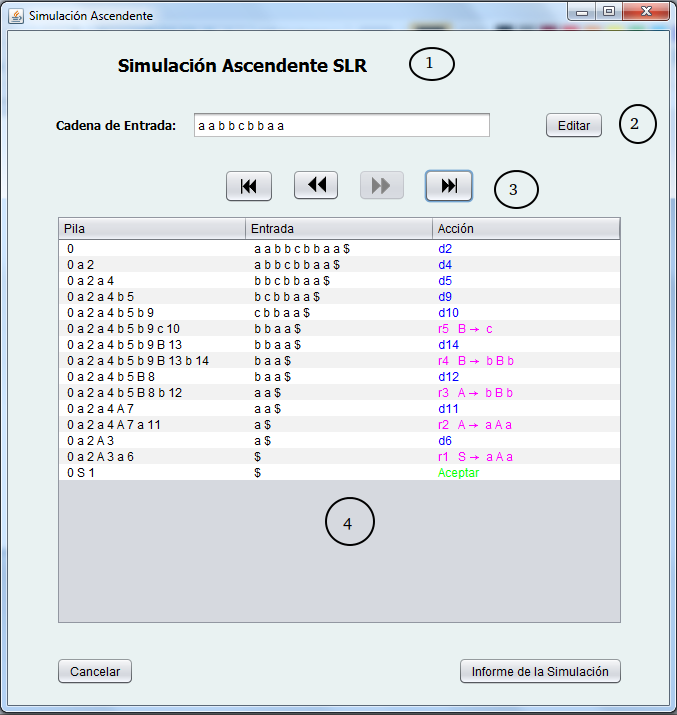
\includegraphics[width=0.7\textwidth]{figuras/Cap10/da14.png}
% 	\caption{ Ventana de simulación}
% 	\label{fig:d7}
%       \end{center}
%   \end{figure}

\section{Ventana de Visualización del Árbol Sintáctico}

% El árbol sintáctico se podrá ver en una ventana la cual se irá repintando a medida que se continue con la simulación (Figura \ref{fig:da22}).

%   \begin{figure}[htp]
%       \begin{center} 
% 	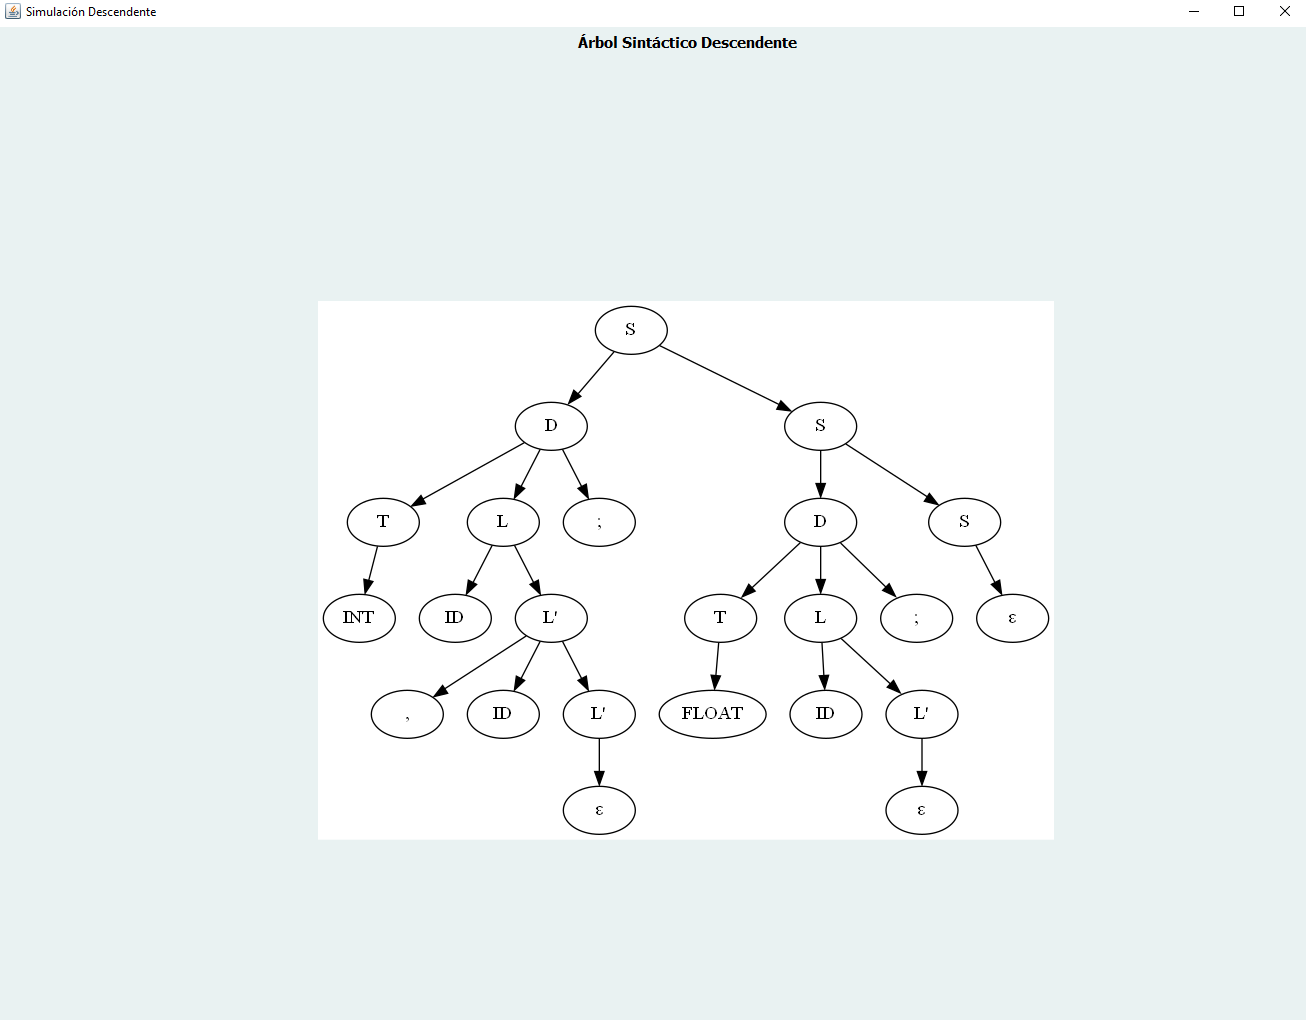
\includegraphics[width=0.7\textwidth]{figuras/Cap10/da22.png}
% 	\caption{ Ventana de simulación}
% 	\label{fig:da22}
%       \end{center}
%   \end{figure}

 \section{Ventana de Derivación Sintáctica}

% Además del árbol, es posible generar la derivación de la simulación actual en una ventana adicional tal y como se muestra en la imagen\ref{fig:da24}:

% \begin{figure}[htp]
%       \begin{center} 
% 	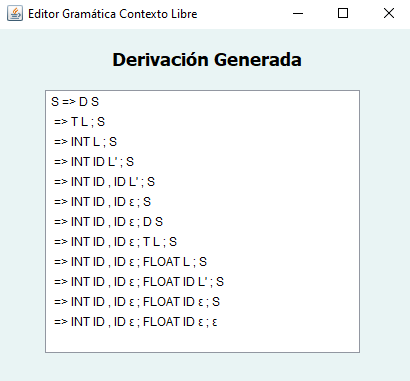
\includegraphics[width=0.7\textwidth]{figuras/Cap10/da24.PNG}
% 	\caption{ Ventana de simulación}
% 	\label{fig:da24}
%       \end{center}
%   \end{figure}

\section{Ventana de asistente}

% En SimAS se han creado dos tipos de asistentes: el \textit{asistente de creación de una gramática} y el \textit{asistente de creación de una simulación}. En la figura \ref{fig:d8}, se muestra un ejemplo de esta ventana; en concreto, el primer paso del asistente de creación de una gramática.

% La ventana está compuesta de los siguientes elementos:
% \begin{enumerate}
%  \item \textbf{Título}: contiene un título descriptivo de la ventana en la que se sitúe el asistente.
%  \item \textbf{Contenido}: información que se muestra en el panel en función del paso en el que se está.
%  \item \textbf{Botonera}: permite controlar la evolución del asistente (cancelar, ir
% al paso anterior, ir al primer paso, etcétera).

% \end{enumerate}

%   \begin{figure}[htp]
%       \begin{center} 
% 	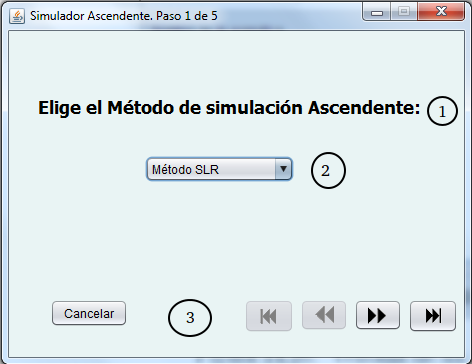
\includegraphics[width=0.6\textwidth]{figuras/Cap10/da16.png}
% 	\caption{ Ventana de asistente.}
% 	\label{fig:d8}
%       \end{center}
%   \end{figure}

\section{Ventanas de edición}

% Las ventanas de edición representa a todas las ventanas que permiten realizar una edición de un objeto (nombre, descripción, símbolos, producciones, funciones de error, etcétera). En la figura \ref{fig:d9}, se muestra un ejemplo de esta ventana; en concreto, la ventana de edición de los símbolos de la gramática.

% La ventana está compuesta de los siguientes elementos:
% \begin{enumerate}
%  \item \textbf{Título}: contiene un título descriptivo de la ventana.
%  \item \textbf{Contenido}: información a editar que se muestra en la ventana.
%  \item \textbf{Botonera}: permite cancelar o aceptar la operación. El botón
% de cancelar siempre estará situado a la izquierda, mientras que el de
% aceptar lo estará en la derecha.

% \end{enumerate}

%   \begin{figure}[htp]
%       \begin{center} 
% 	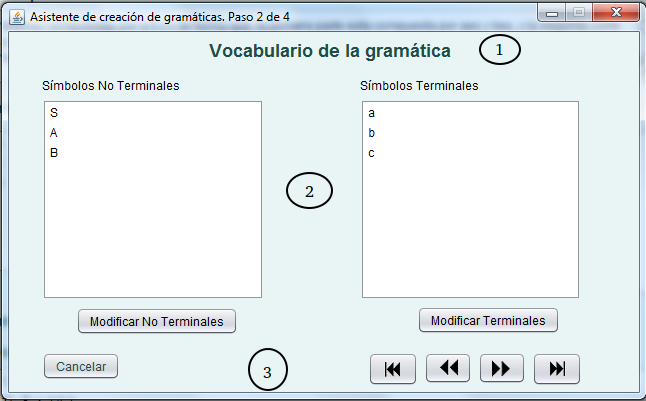
\includegraphics[width=0.7\textwidth]{figuras/Cap10/da18.png}
% 	\caption{ Ventana de edición.}
% 	\label{fig:d9}
%       \end{center}
%   \end{figure}
